\chapter{Appendix to Chapter 5}
\label{chap:appendix_ch5}

\section{Simulation Details for Results in Section \ref{subsec:tparam_motivation}}
\label{sec:tparam_motiv_details}

\subsection{Simulation setup}
\label{subsec:tparam_motiv_setup}

We simulated an outbreak with SIRS dynamics in a population of $ N= 100,000$ individuals, ten of whom were initially infected, spanning two wave of the outbreak over thirty weeks. The mean infectious period duration was one week, and the mean duration of immunity was four weeks. The basic reproduction numbers of the outbreak, and hence the per--contact infectivity rates, varied sinusoidally with additive noise, over the course of the outbreak:
\begin{equation}
\label{eqn:sinfoi_true_R0t}
R0(t) = \beta(t) N / \mu = 2 + 0.35(\sin(t / 3.5) + 0.1Z_t),
\end{equation} 
where $ Z_t \sim N(0,1)$. The per--contact infection rates were then obtained as $ \beta(t) = R0(t) \mu / N $ The observed incidence was a negative binomial sample of the true incidence with mean case detection rate $ \rho $ and overdispersion parameter $ \phi $: 
\begin{equation}
Y_\ell \sim \mr{Neg.Binom.}\left (\mu  = \rho(N_{SI}(t_\ell) - N_{SI}(t_{\ell-1})), \sigma^2 = \mu(1 + \mu /\phi) \right ).
\end{equation}

We fit two models, one where the force of infection was constant over the course of the outbreak and another where the rates of infectious contact were time varying, with log--differences in the basic reproduction numbers penalized using a first order Gaussian Markov random field (GMRF) shrinkage prior where the standard deviation of the log--differences is given by $ \sigma_{RW1} $ (analogous to the models in Section \ref{sec:flu_tparam_models}). We employed non--centered parameterizations for both the LNA and the GMRF. The models were fit under informative priors, summarized in Table \ref{tab:tparam_sim_priors}. We ran five MCMC chains per model for 100,000 iterations per chain, alternating between five elliptical slice sampling (EllipSS) updates and one multivariate normal slice sampling (MVNSS) updates per MCMC iteration. The estimation scale on which the MCMC explored the parameter space was given by $\lbrace \log(R0(t_0)), \log(1/mu), \logit(\rho), 1/\sqrt(\phi) \rbrace$. The MVNSS proposal covariance matrix was adapted throughout the first 50,000 iterations, samples from which were subsequently discarded, using the gain factor sequence: the gain factor sequence, $\gamma_n = 0.5(1 + 0.01n)^{-0.99}$. The contribution of isotropic Gaussian noise to the MVNSS proposal was initialized at 0.001 and reduced throughout the adaptation phase according to the sequence $ \iota_n = 0.001(1 + 0.01n)^{-0.99} $. Convergence was assessed visually by inspection of traceplots of posterior samples, and via potential scale reduction factors (PSRFs) \cite{brooks1998general} computed via the \texttt{coda} R package \cite{codapackage}.

\begin{table}[htbp]
	\caption[Parameters and priors for models fit two SIRS models to data from a simulated outbreak with sinusoidal FOI.]{Parameters and priors used in fitting two SIRS models, one with constant FOI and another with time--varying FOI, to data from an outbreak with SIRS dynamics where the per--contact infection rate varied sinusoidally over time.}
	\label{tab:tparam_sim_priors}
	\scriptsize\centering
	\begin{tabular}{clllr}
		\hline
		\textbf{Parameter} & \textbf{Interpretation} & \textbf{Truth} & \textbf{Prior} & \textbf{Median (95\% Interval)} \\ \hline
		$ R0-1 $ & Basic reproduction \#-1 & (\ref{eqn:sinfoi_true_R0t}) & LogNormal(0, 0.5) & $ \implies R0(t_0) = $ 2.00 (1.14, 8.10) \\ 
		$ 1/\mu $ & Mean infectious period & 1&  LogNormal(0.05, 0.5)& 1.05 (0.39, 2.80) \\
		$ \rho/(1-\rho)  $ & Odds of case detection  &0.25&  LogNormal(-0.847, 0.5) & $ \implies \rho =$ 0.3 (0.14, 0.53) \\
		$ 1/\sqrt{\phi} $ & Neg.Binom. overdispersion & 50 & Exponential(5)& $ \implies \phi = 52 (1.84, 39000) $.  \\
		\hline
	\end{tabular}
\end{table}

\newpage
\subsection{Additional results}
\label{subsec:sinfoi_supp_res}

\begin{figure}[htbp]
	\centering
	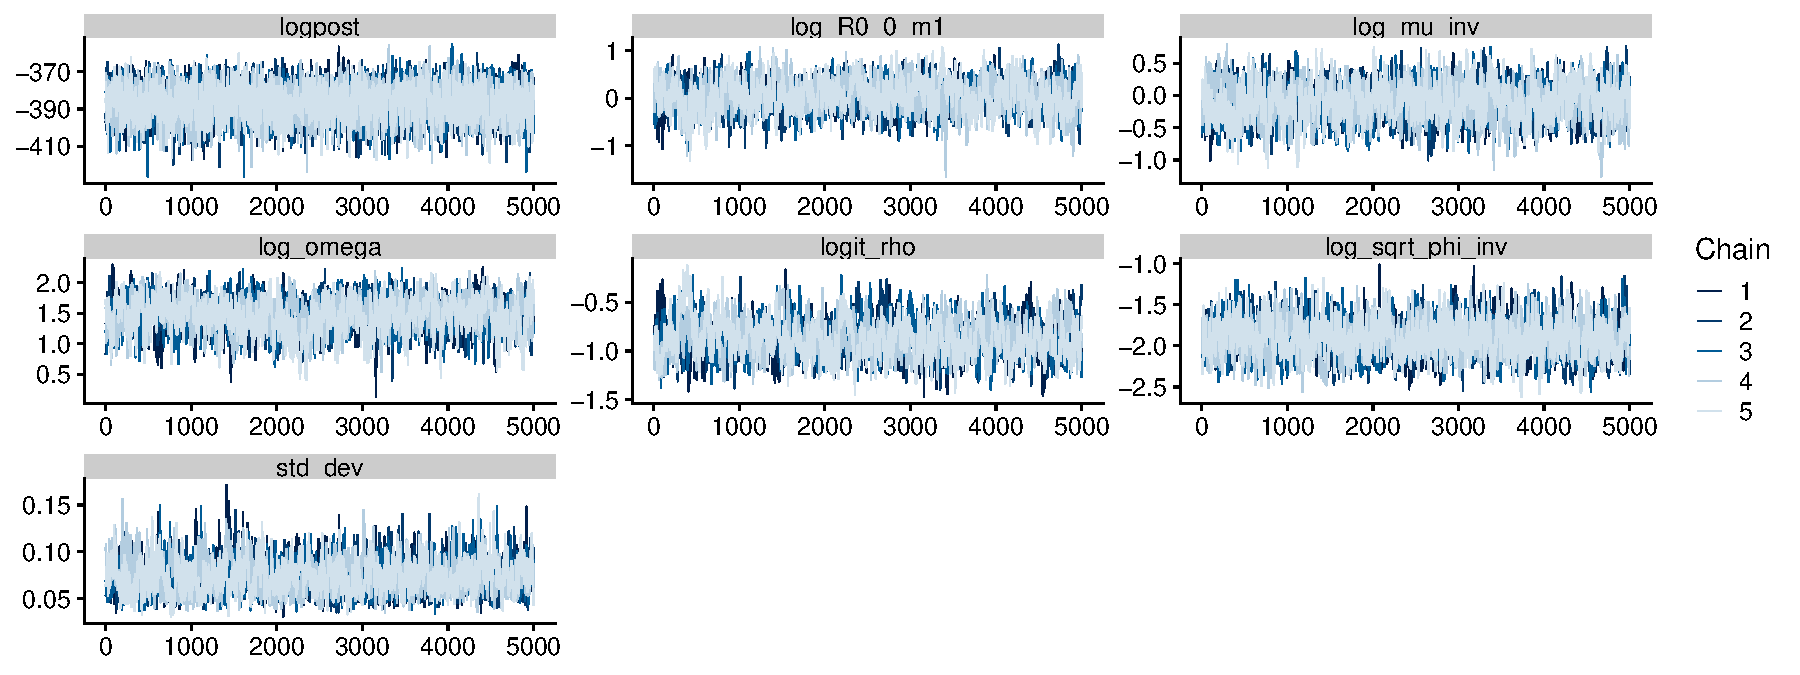
\includegraphics[width=\linewidth]{figures/sinfoi_rw1_traces}
	\caption{Posterior traceplots for SIRS model parameters with time--varying force of infection.}
	\label{fig:sinfoirw1traces}
\end{figure}

\begin{figure}[htbp]
	\centering
	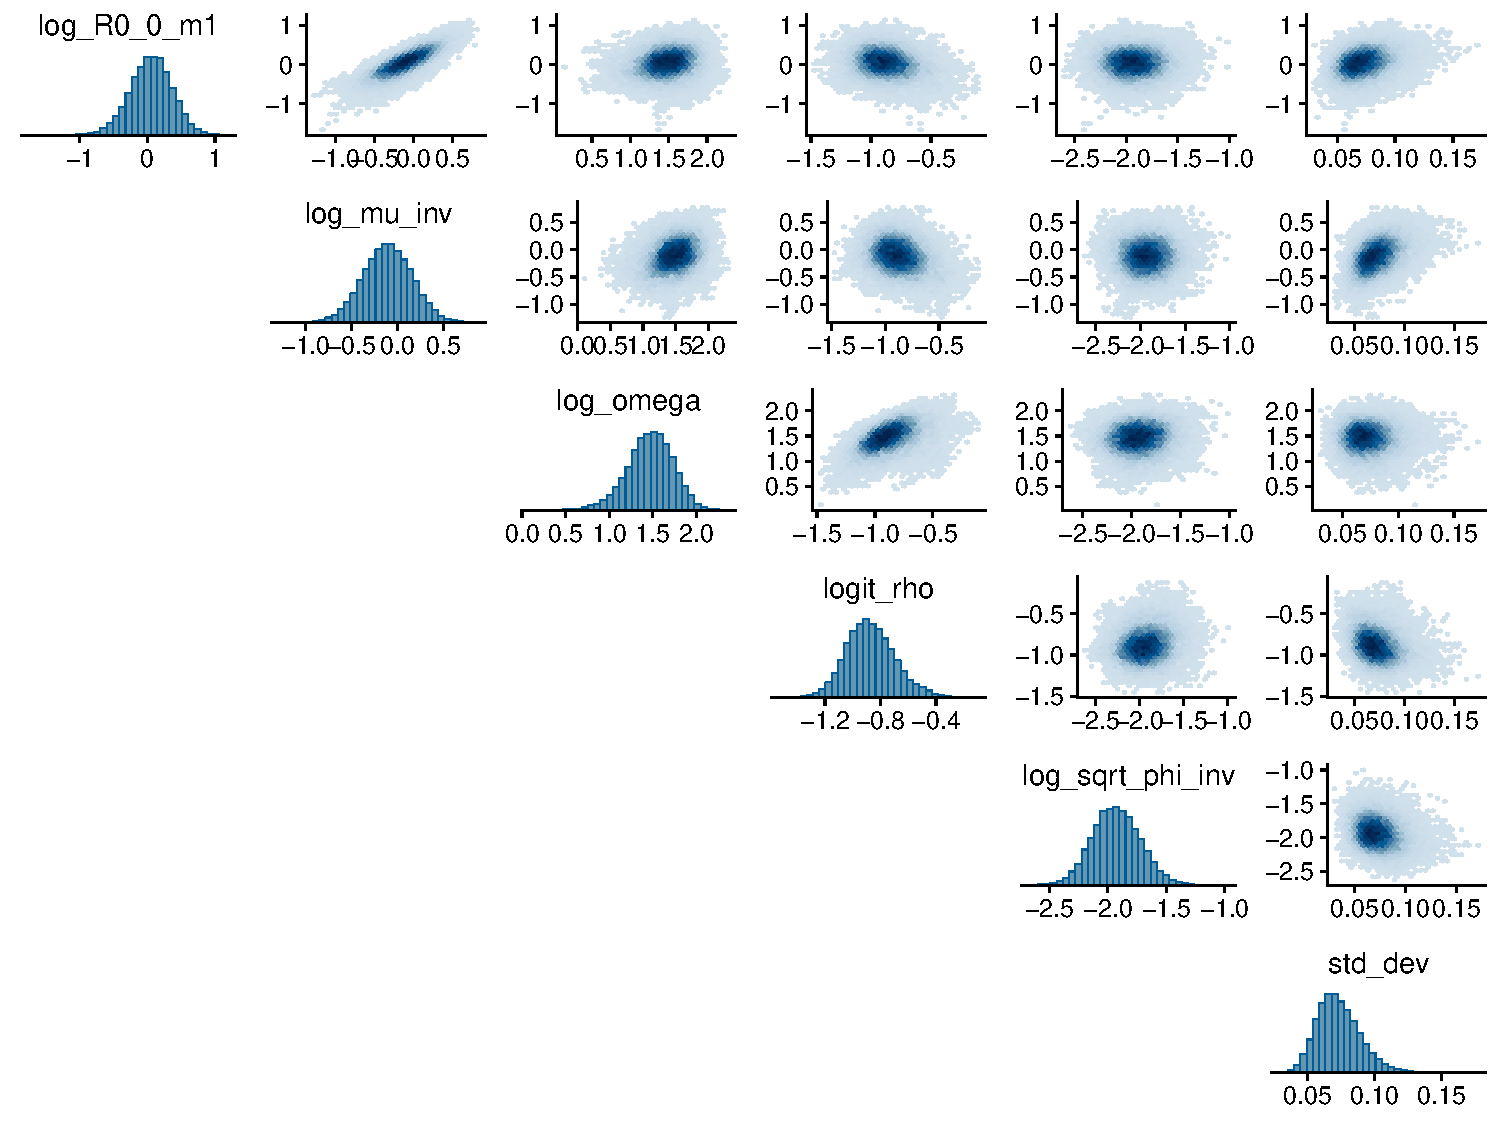
\includegraphics[width=\linewidth]{figures/sinfoi_rw1_pairs}
	\caption{Posterior histograms and pairwise hexplots for SIRS model parameters with time--varying force of infection.}
	\label{fig:sinfoirw1pairs}
\end{figure}

\begin{figure}[htbp]
	\centering
	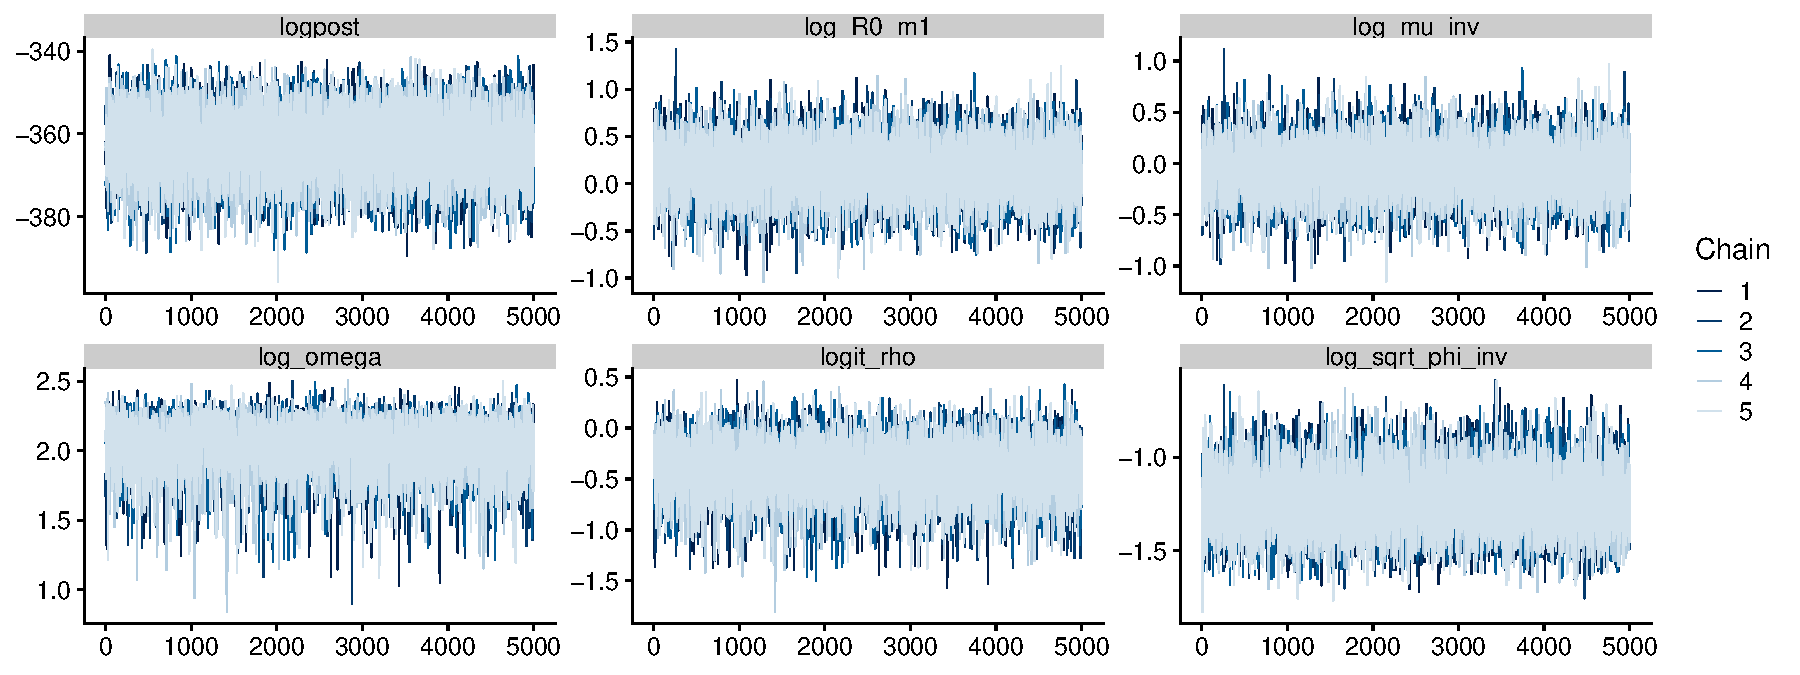
\includegraphics[width=\linewidth]{figures/sinfoi_const_traces}
	\caption{Posterior traceplots for SIRS model parameters with time--homogeneous force of infection.}
	\label{fig:sinfoiconsttraces}
\end{figure}

\begin{figure}[htbp]
	\centering
	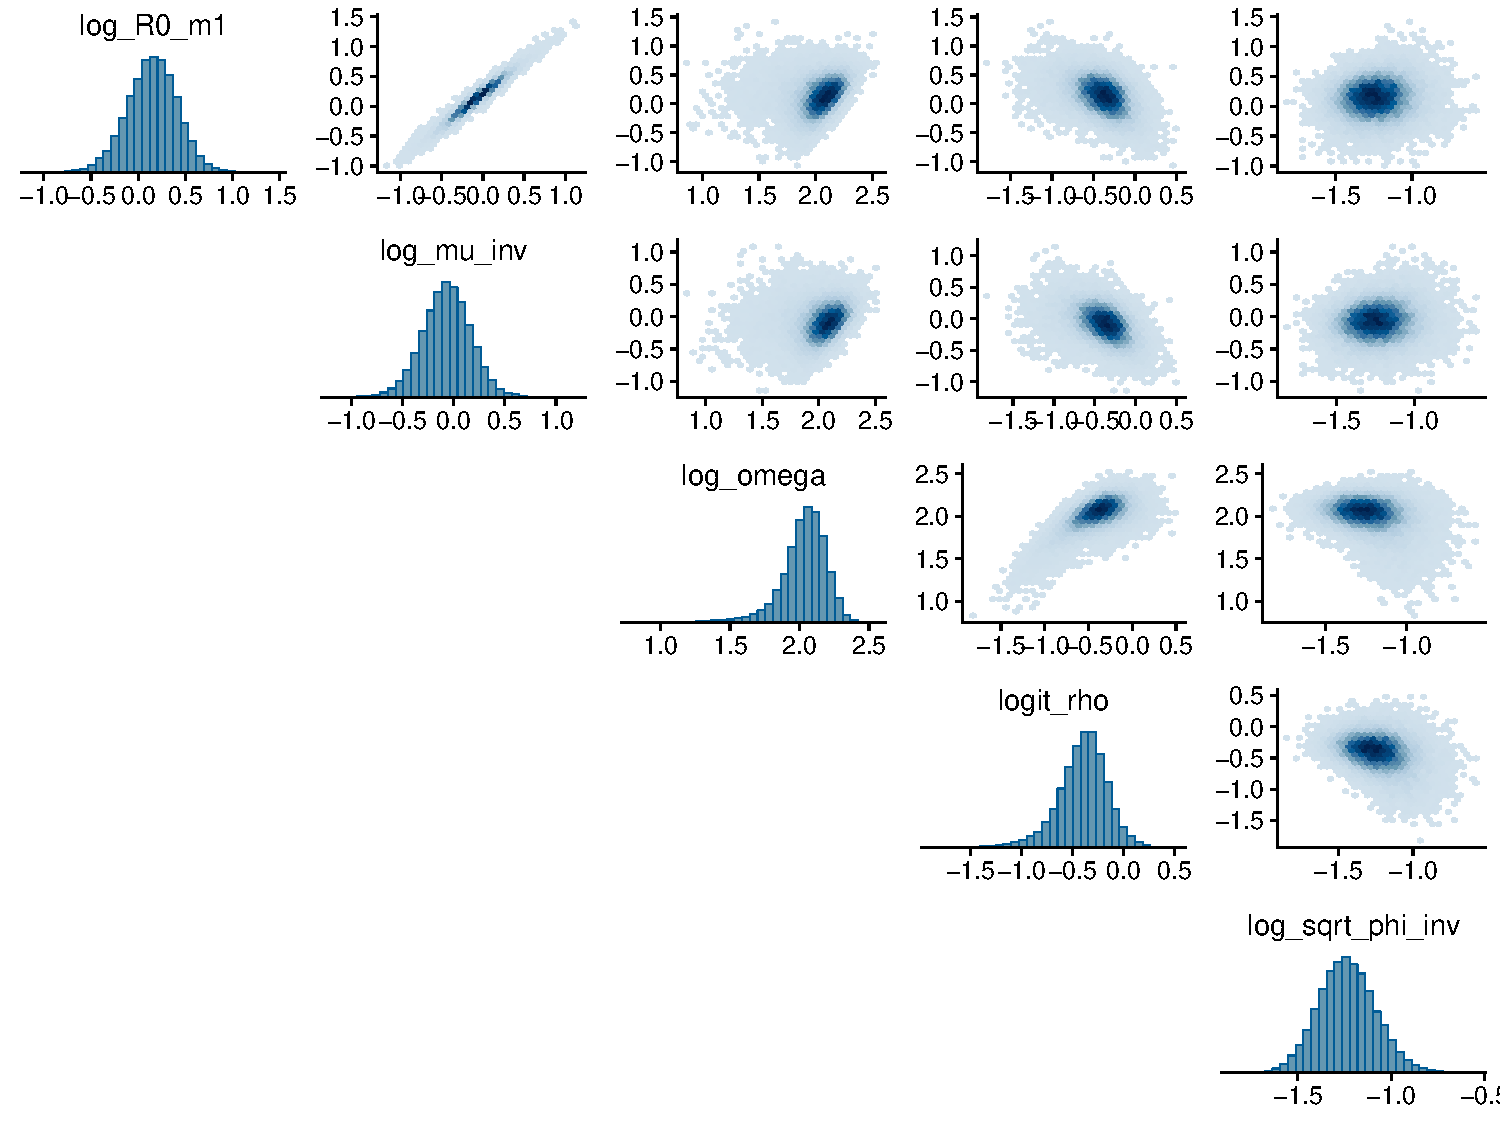
\includegraphics[width=\linewidth]{figures/sinfoi_const_pairs}
	\caption{Posterior histograms and pairwise hexplots for SIRS model parameters with time--homogeneous force of infection.}
	\label{fig:sinfoiconstpairs}
\end{figure}

\begin{figure}[htbp]
	\centering
	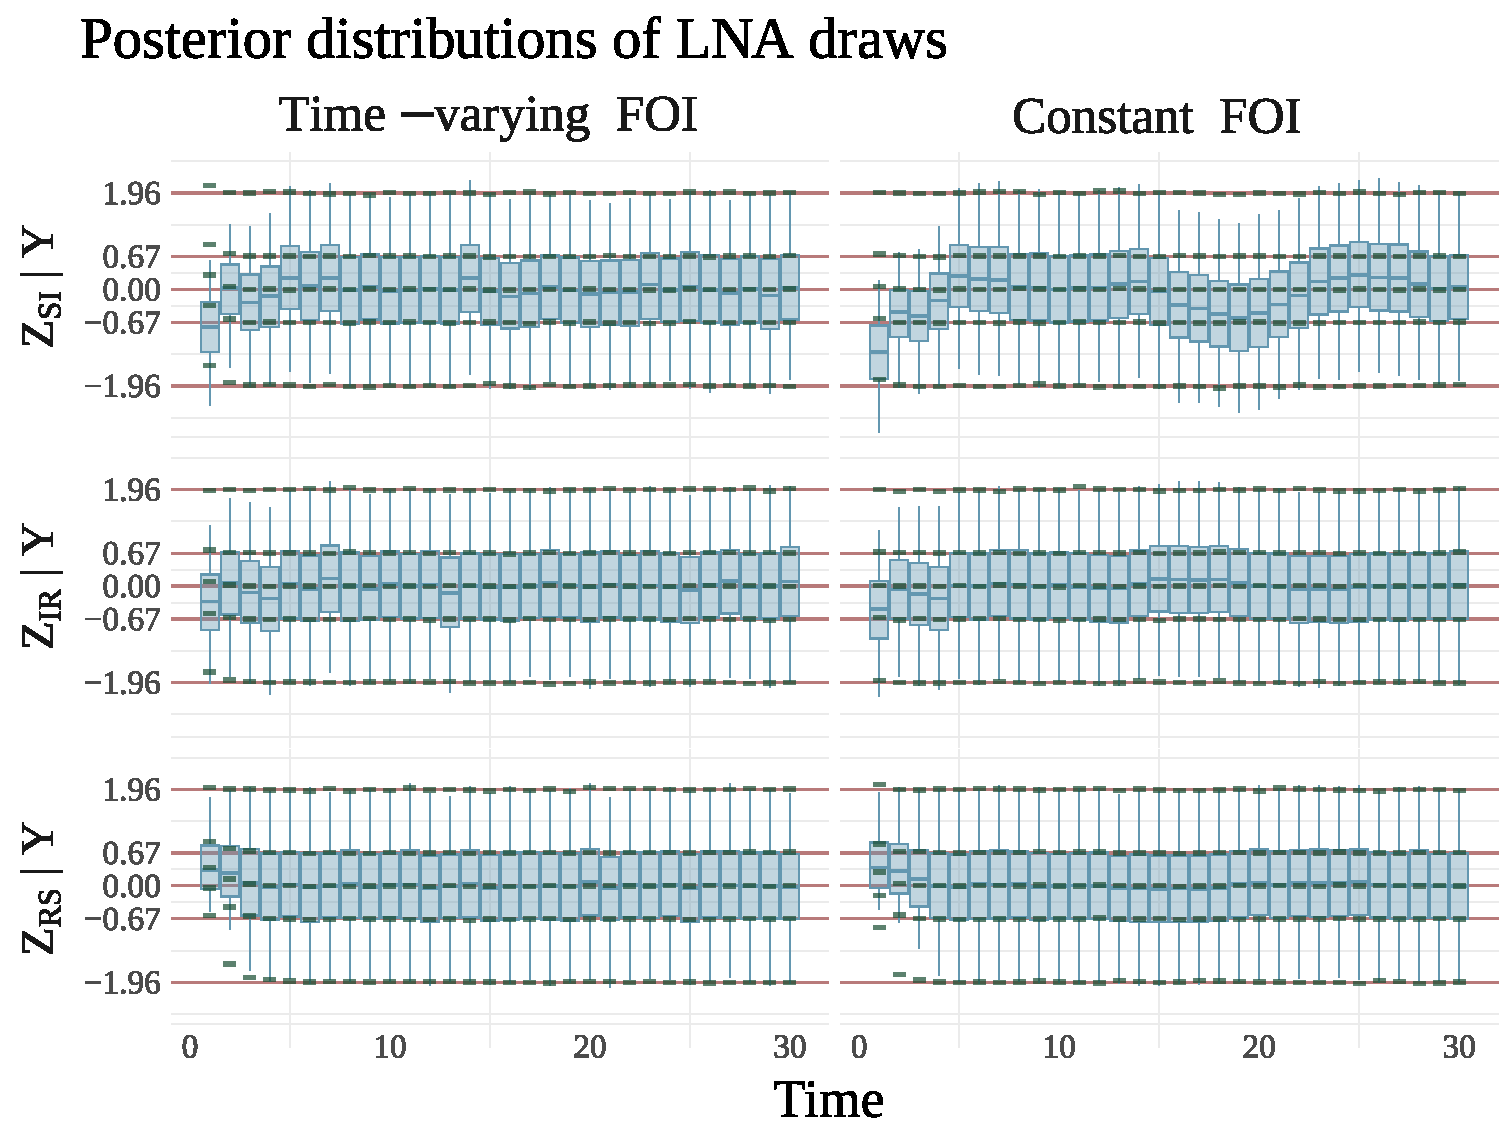
\includegraphics[width=\linewidth]{figures/sinfoi_lna_drawplots}
	\caption[Posterior distributions of LNA draws for SIRS models with time--varying and constant force of infection.]{Posterior distributions of the LNA draws for infection, recovery, and loss of immunity in SIRS models with time--varying and constant force of infection (blue boxplots). The lower and upper whisker tips correspond to the $ 2.5^\mr{th} $ and $ 97.5^\mr{th} $ posterior quantiles, the lower and upper hinges to the $ 25^\mr{th} $ and $ 75^\mr{th} $ quantiles, and the middle hash mark to the posterior median. The solid red lines are the theoretical quantiles of the posterior predictive distribution (or equivalently, the prior distribution) of the LNA draws, drawn at the quantiles of a standard normal distribution corresponding to the boxplot quantiles. The green ticks are the estimated quantiles of the posterior predictive distributions of the LNA draws, accounting for boundary conditions on the state space of the latent process and obtained by simulating LNA paths from the posterior predictive distribution. The posterior distributions of LNA draws are shaded according to the level of posterior shrinkage, computed as one minus the ratio of standard deviations of LNA draws in the posterior and prior.}
	\label{fig:sinfoidrawplots}
\end{figure}

\newpage
\section{Specification of Contact Rates}
\label{sec:flu_contact_rates}

Contact rates within and between age--strata were obtained from the Finnish arm of the POLYMOD survey \cite{mossong2008social,polymod}, and were accessed via the \texttt{socialmixr R} package \cite{funk2018socialmixr}. The survey was a population--based, prospective survey that recorded contact rates by sex, age, location, duration, and frequency. We queried the symmetric form of the estimated mean contact matrix aggregated age--strata in our analysis (0--19 years and 20+ years), which based on a sample of 1,006 individuals. A contact matrix is said to be symmetric if the total number of contacts between two groups is equal. In particular, if $ c_{ij} $ is the mean number of contacts an individual in group $ i $ has with members of group $ j $, and group $ i $ is of size $ N_i $, then symmetry requires that $ c_{ij}N_i = c_{ji}N_j $. Due to the vagaries of sampling variability, this relation does not always hold. The symmetric contact matrix is obtained by taking $ c_{ij}^{\prime} = (c_{ij}N_i + c_{ji}N_j) / 2N_i $. 

The estimated mean contact rates are
\[ \bC_{tot} = 
\kbordermatrix{
	 & 0-19 & 20+ \\
	 0-19 & 7.44 & 5.05 \\
	 20+ & 1.55 & 8.56
}. \]
Following \cite{meyer2017incorporating}, we row--normalize the matrix, thus removing differences in absolute contact rates. This is helpful in parameterizing and assigning sensible priors to other aspects of the model, such as basic reproduction numbers. The normalized contact rates are
\[ \bC = 
\kbordermatrix{
	& 0-19 & 20+ \\
	0-19 & 0.60 & 0.40 \\
	20+ & 0.15 & 0.85
}. \]

\section{Mapping Standard Normal Draws to LNA Sample Paths with Forcings}
\label{sec:dolna_forcings}
\begin{algorithm}[htbp]
	\caption{Mapping standard normal draws onto LNA sample paths with forcings.}
	\label{alg:doLNA2}
	\begin{algorithmic}[1]
		\Procedure{doLNA2}{$ \bZ,\btheta,\mcI,\bxi $}
		\State \textbf{initialize: }$ \bX(t_0) \gets \bX_0,\ \bN(t_0) \gets \bs{0},\ \bNtil(t_0) \gets \bs{0},\ \bmu(t_0) \gets \bs{0},\ \bSigma(t_0) \gets \bs{0} $
		\For{$ \ell = 1,\dots,L $}
		\State $ \bmu(t_\ell),\ \bSigma(t_\ell) \gets $ solutions to (\ref{eqn:lna_ode_drift}) and (\ref{eqn:lna_ode_diffusion}) over $ (t_{\ell-1}, t_\ell] $
		\State $ \bNtil(t_\ell)\gets \bmu(t_\ell) + \bSigma(t_\ell)^{1/2}\bZ(t_\ell) $ \Comment{non--centered parameterization}
		\State $ \bN(t_\ell)\gets \bN(t_{\ell-1}) + \exp(\bNtil(t_\ell)) - \bs{1} $
		\State \textbf{restart initial conditions:} 
		  \vspace{-0.15in}\hspace{0.2in} \begin{align*}
			\bX(t_\ell) &\gets \bX(t_{\ell-1}) + \bA^T(\bN(t_\ell)-\bN(t_{\ell-1})) \\
			\bX(t_\ell^+) &\gets \bX(t_\ell) + \bxi(t_\ell)\\
			\bNtil(t_\ell) &\gets \bs{0},\ \bmu(t_\ell)\gets\bs{0},\ \bSigma(t_\ell)\gets\bs{0}
			\end{align*}\vspace{-0.35in}
		\EndFor
		\State \hspace{-0.25in}\Return \Comment{return incidence and/or prevalence sample paths}
		\State$\bN = \left \lbrace\bN(t_0),\bN(t_1),\dots,\bN(t_L)\right \rbrace,\ \bX = \left \lbrace \bX(t_0),\ \bX(t_1),\dots,\bX(t_\ell) \right \rbrace $
		\EndProcedure
	\end{algorithmic}
\end{algorithm}

\newpage
\section{Joint Sampling of LNA Paths and Gaussian Markov Random Fields}
\label{sec:lna_ess_gmrf}

Jointly sampling the LNA draws and the values of a GMRF, $ \bF $, in addition to possibly any other latent Gaussian parameters including the initial compartment volumes as in Section \ref{sec:lna_init_volumes}, requires trivially modifying Algorithm \ref{alg:elliptss_lna_initvols} to include the additional parameters. We implement the same computational strategy used throughout Chapters \ref{chap:lna_for_sems} and \ref{chap:lna_extensions} of using non--centered parameterizations for the parameters of interest and the LNA path. As we have noted, this has the advantage of breaking the autocorrelation that would otherwise lead to poor MCMC mixing when using a centered parameterization and alternating between updates to different parameters in the model. We will denote by $ \bZ = (\bZ^X,\ \bZ^{X_0},\ \bZ^F,\ \bZ^{\btheta_F}) $ the multivariate standard normal draws for the latent LNA process, the initial compartment volumes, the draws to be mapped to the GMRF, and $ \bZ^{\btheta_F} $ the draws that are mapped to the GMRF hyper--parameters that are to be updated along with the GMRF. Unless otherwise stated (and we never do so state), we will at the very least update the precision or standard deviation of the GMRF increments jointly with the field to avoid poor MCMC mixing. We will assume that non--centered parameterizations for the GMRF and the hyper--parameters are linear transformations and thus do not require Jacobian terms to be included in the ElliptSS acceptance probability. We will denote by $ \bm_0 $, $ \bm_\theta $, $ \bV_0 $, and $ \bV_\theta $ the means and covariance matrices of the initial volumes and hyper--parameters, and by $ \doGMRF $ the linear operator for mapping $ \bZ^F $ to a GMRF sample, i.e., the GMRF values are obtained by $ \doGMRF(\bZ^F; \btheta_F) $. 

\begin{algorithm}[htbp]
	\caption{Sampling LNA draws, initial volumes, GMRF values, and GMRF hyper--parameters via elliptical slice sampling.}
	\label{alg:elliptss_lna_gmrf}
	\begin{algorithmic}[1]
		\Procedure{\doElliptSS3}{$ \bZ = (\bZ^X_{cur}, \bZ^{X_0}_{cur},\bZ^{F},\bZ^{\btheta_F}),\btheta,\bY,\mcI,\omega = 2\pi $}
		\State Sample ellipse: $ \bZ_{prop} \sim N(\bs{0}, \mb{I})$
		\State Sample threshold: $ u|\bx \sim \mr{Unif}(0, L(\bY|\doLNA(\bZ_{cur},\btheta,\mcI))) $
		\State Position the bracket: \vspace{-0.15in}
		\begin{align*}
		\psi &\sim \mr{Unif}(0,\omega)\\
		L_\psi &\leftarrow -\psi;\ R_\psi \leftarrow L_\psi + \psi\\
		\phi &\sim \mr{Unif}(L_\psi,R_\psi)
		\end{align*}
		\State Compute the proposal: \vspace{-0.1in}\begin{align*}
		\bZ^\prime &\leftarrow \bZ_{cur}\cos(\phi) + \bZ_{prop}\sin(\phi) \\
		&\implies \bX_0^\prime = \bm_0 + \bV_0^{1/2}\bZ^{X_0^\prime}\\
		&\implies\btheta_F^\prime = \bm_\theta + \bV_\theta^{1/2}\bZ^{\theta_F^\prime} \\
		&\implies\bF^\prime = \doGMRF(\bZ^F;\btheta_F)
		\end{align*}
		\If{$ L(\bY|\doLNA(\bZ^{X\prime},\bX_0^\prime,\bF^\prime,\btheta_F^\prime,\btheta,\mcI)) > u $}{ accept $ \bZ^\prime $}
		\State\Return{ $ \bZ' $}
		\Else
		\State Shrink bracket and try a new angle:
		\State{\textbf{If:} $ \phi < 0 $}{ \textbf{then: }$ L_\phi \leftarrow\phi $ }{ \textbf{else: }$ R_\phi \leftarrow \phi $}
		\State $ \phi \sim \mr{Unif}(L_\phi, R_\phi) $
		\State \textbf{GoTo:} 5
		\EndIf
		\EndProcedure
	\end{algorithmic}
\end{algorithm}

\section{Modeling Pandemic A(H1N1) Influenza in Finland --- Additional Details and Supplementary Results}
\label{sec:flu_supplement}

\subsection{Prior Specification}
\label{subsec:flu_priors}

\subsubsection{Priors for Time--homogeneous Parameters}
\label{subsubsec:flu_param_priors_homog}

\subsubsection{Priors for GMRFs}
\label{subsubsec:flu_gmrf_priors}

\subsection{MCMC Details}

\label{subsec:flu_mcmc_details}

\subsection{Additional Results}
\label{subsec:flu_additional_results}

\subsubsection{Stratified SIRS model with time--varying dynamics}
\label{subsubsec:flu_additional_res_rw1}

\begin{sidewaysfigure}[htbp]
	\centering
	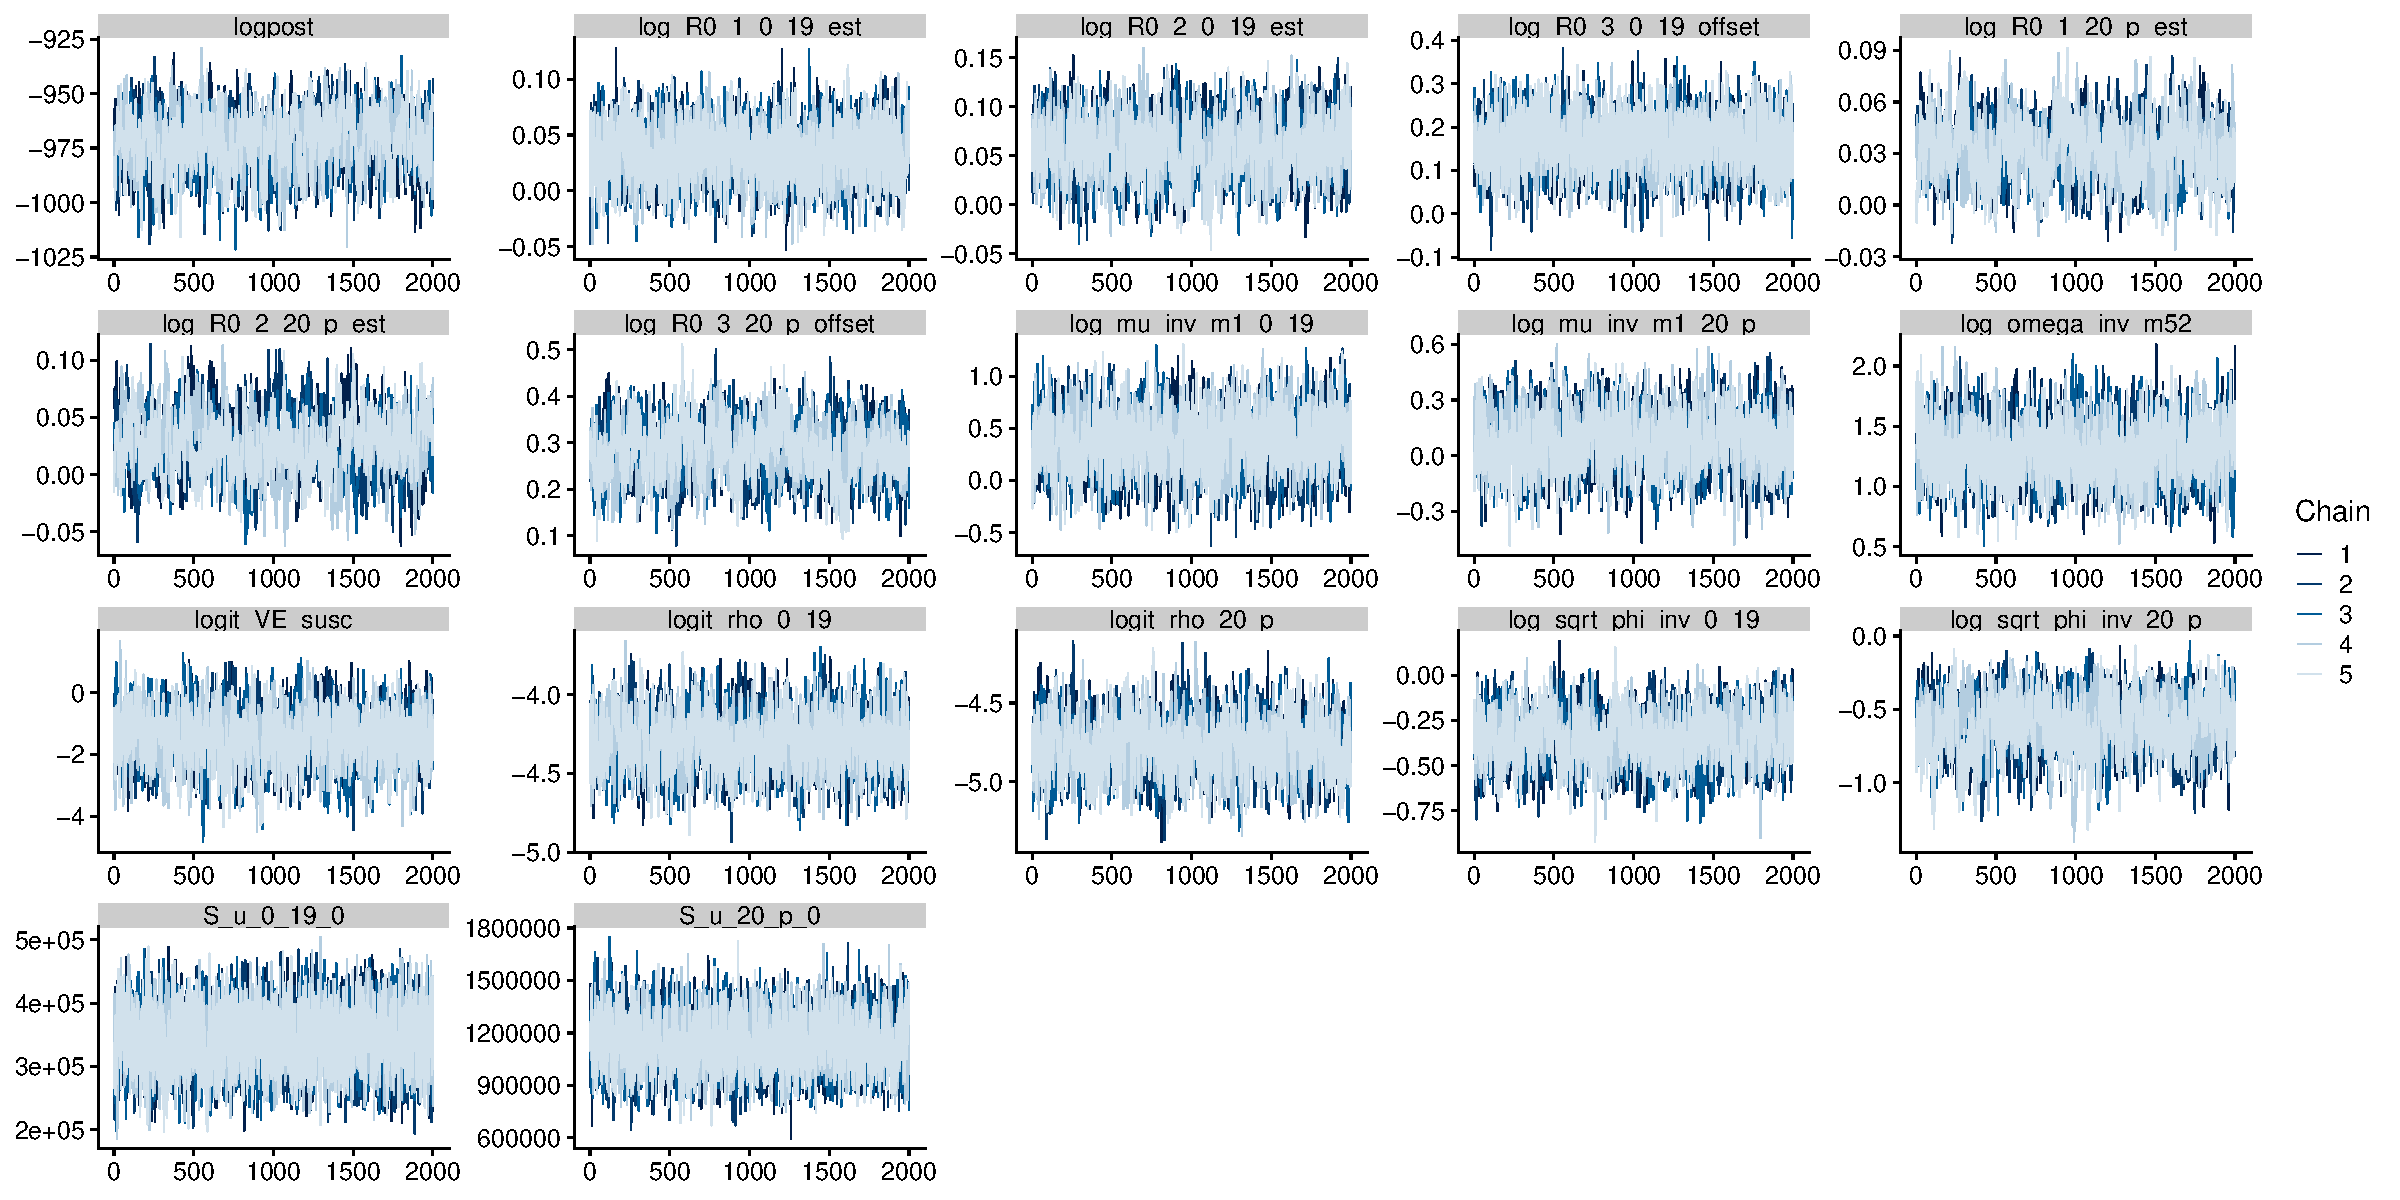
\includegraphics[width=\linewidth]{figures/flu_traces_rw_ode}
	\caption{Posterior traceplots for a stratified SIRS ODE model with time--varying dynamics fit to data from the A(H1N1) influenza pandemic in Finland.}
	\label{fig:flutracesrwode}
\end{sidewaysfigure}

\begin{sidewaysfigure}[htbp]
	\centering
	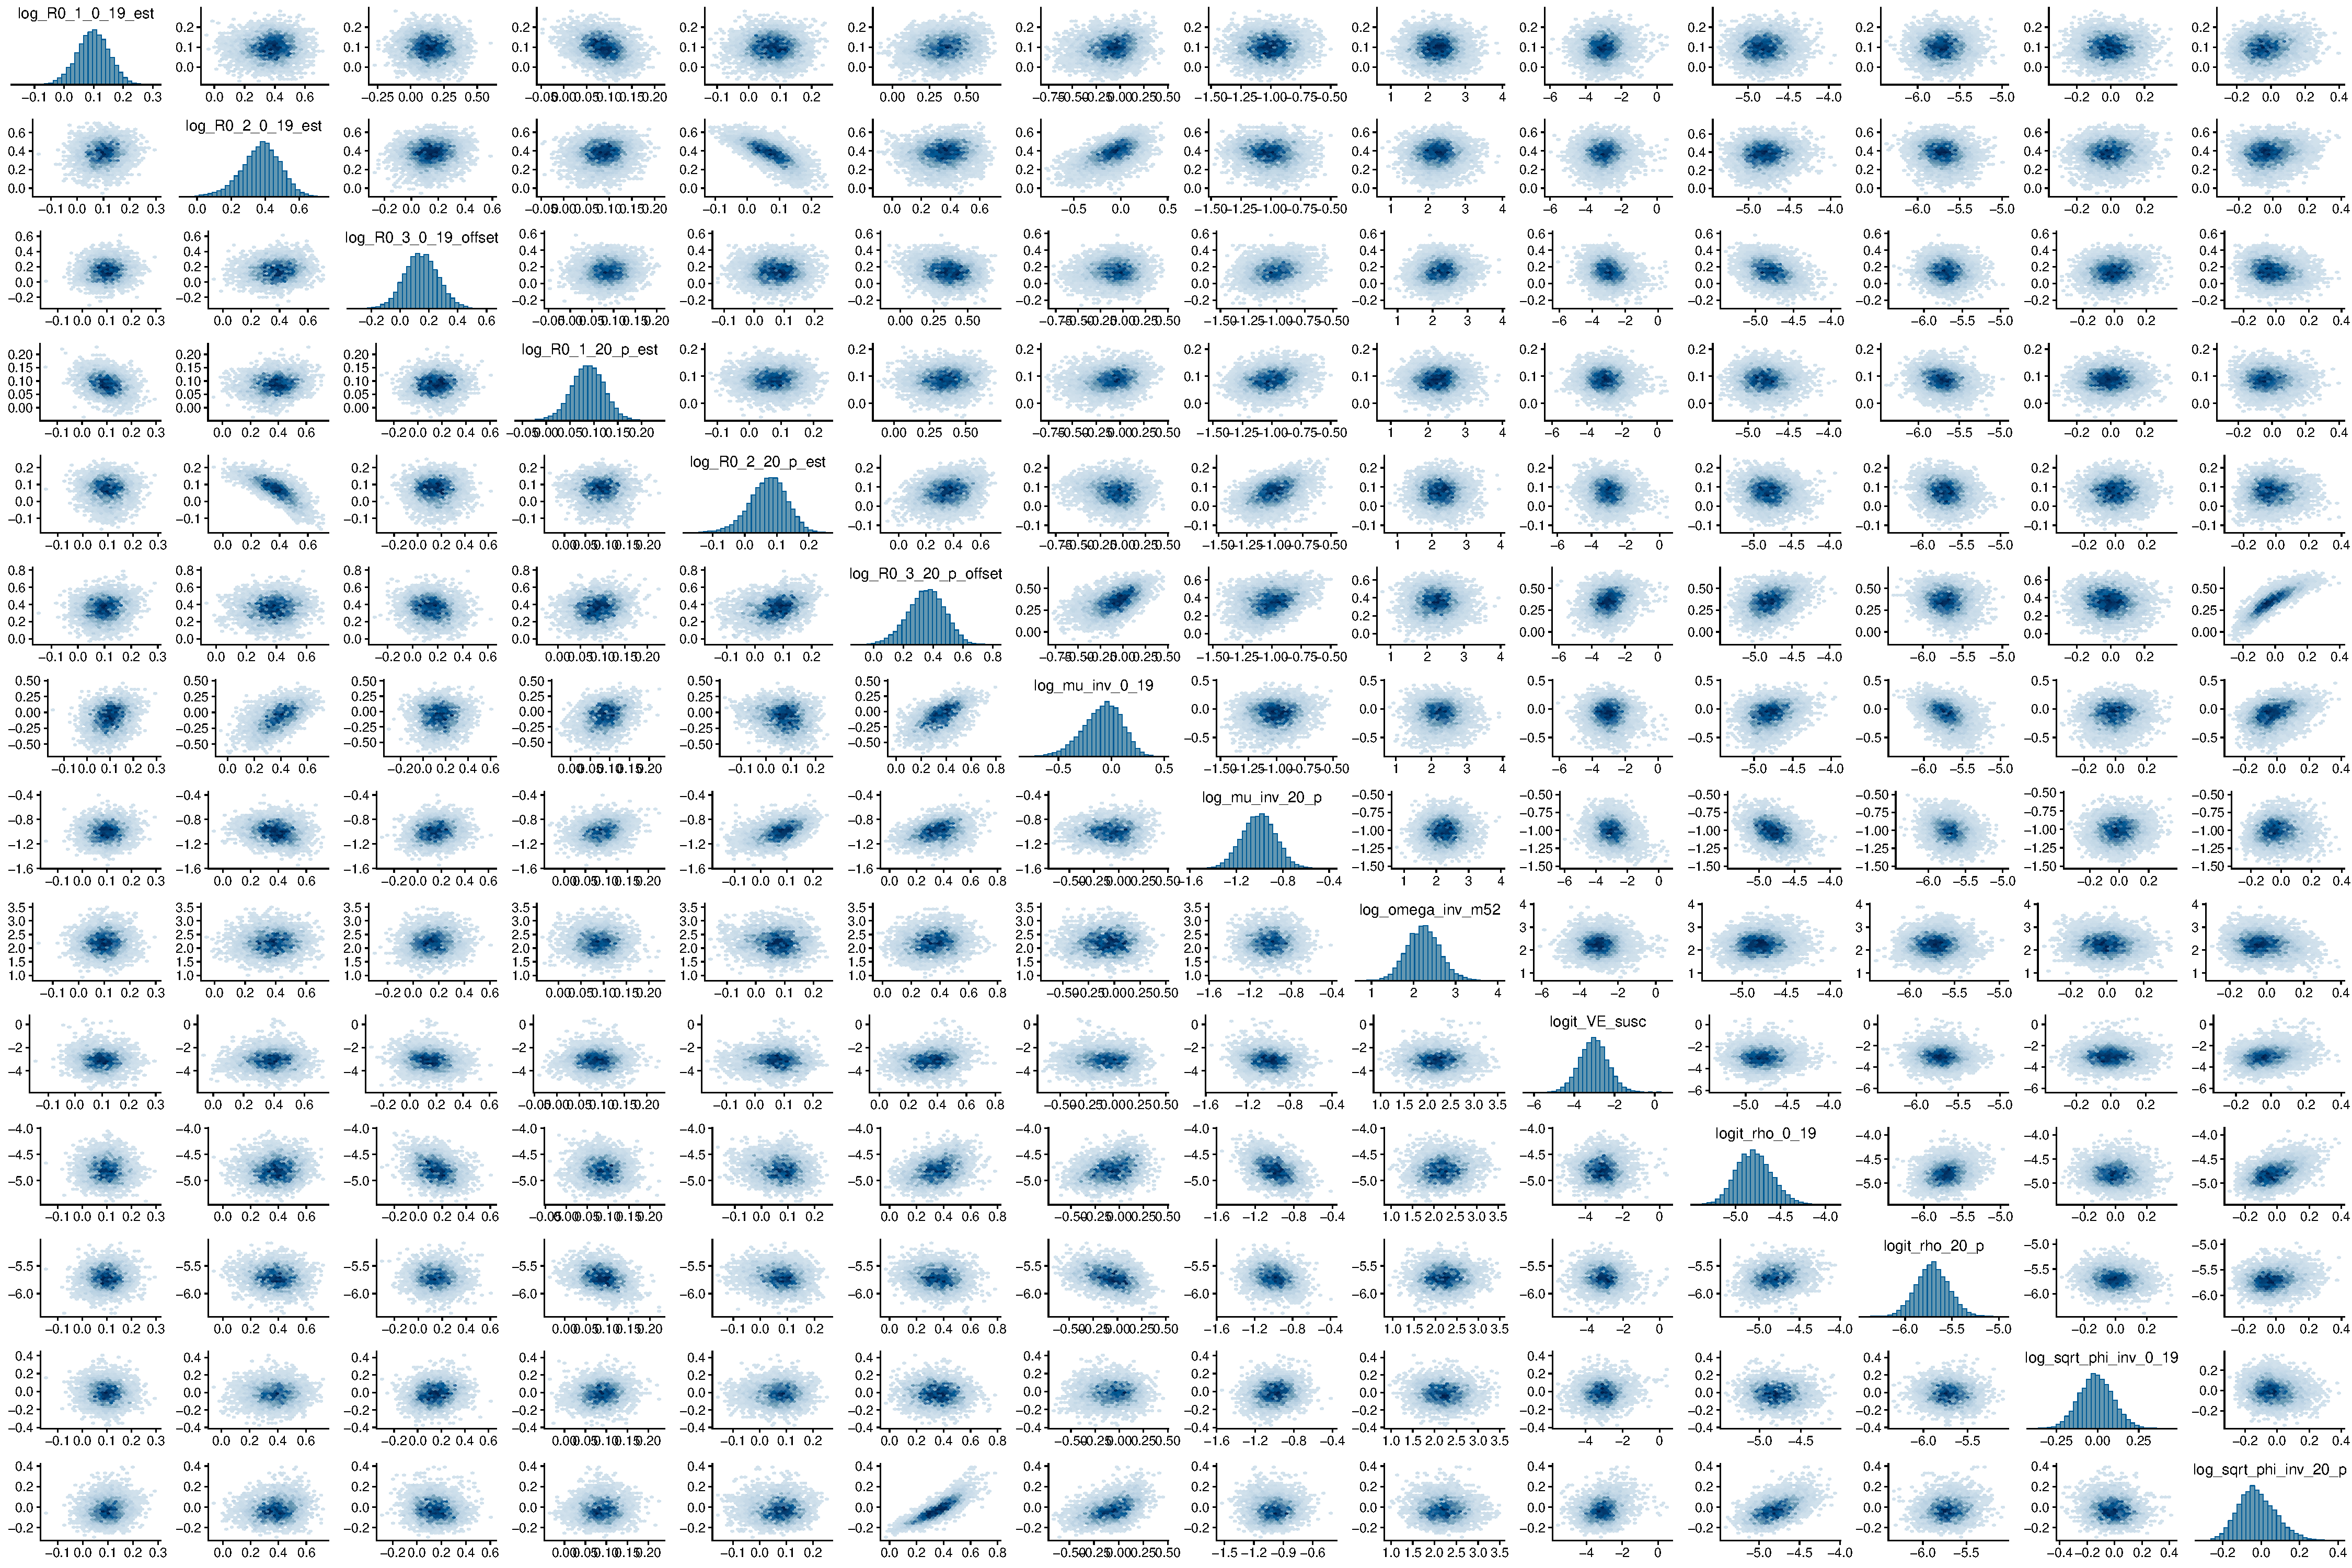
\includegraphics[width=\linewidth]{figures/flu_rw_pairs}
	\caption{Histograms and pairwise scatterplots of posterior samples for the parameters of a stratified SIRS ODE model with time varying dynamics that were sampled via MVNSS. The model was fit to data from the A(H1N1) influenza pandemic in Finland.}
	\label{fig:flurwpairs}
\end{sidewaysfigure}

\newpage

\subsubsection{Stratified SIRS model with piecewise--homogeneous dynamics}
\label{subsubsec:flu_additional_res_const}

\begin{sidewaysfigure}[htbp]
	\centering
	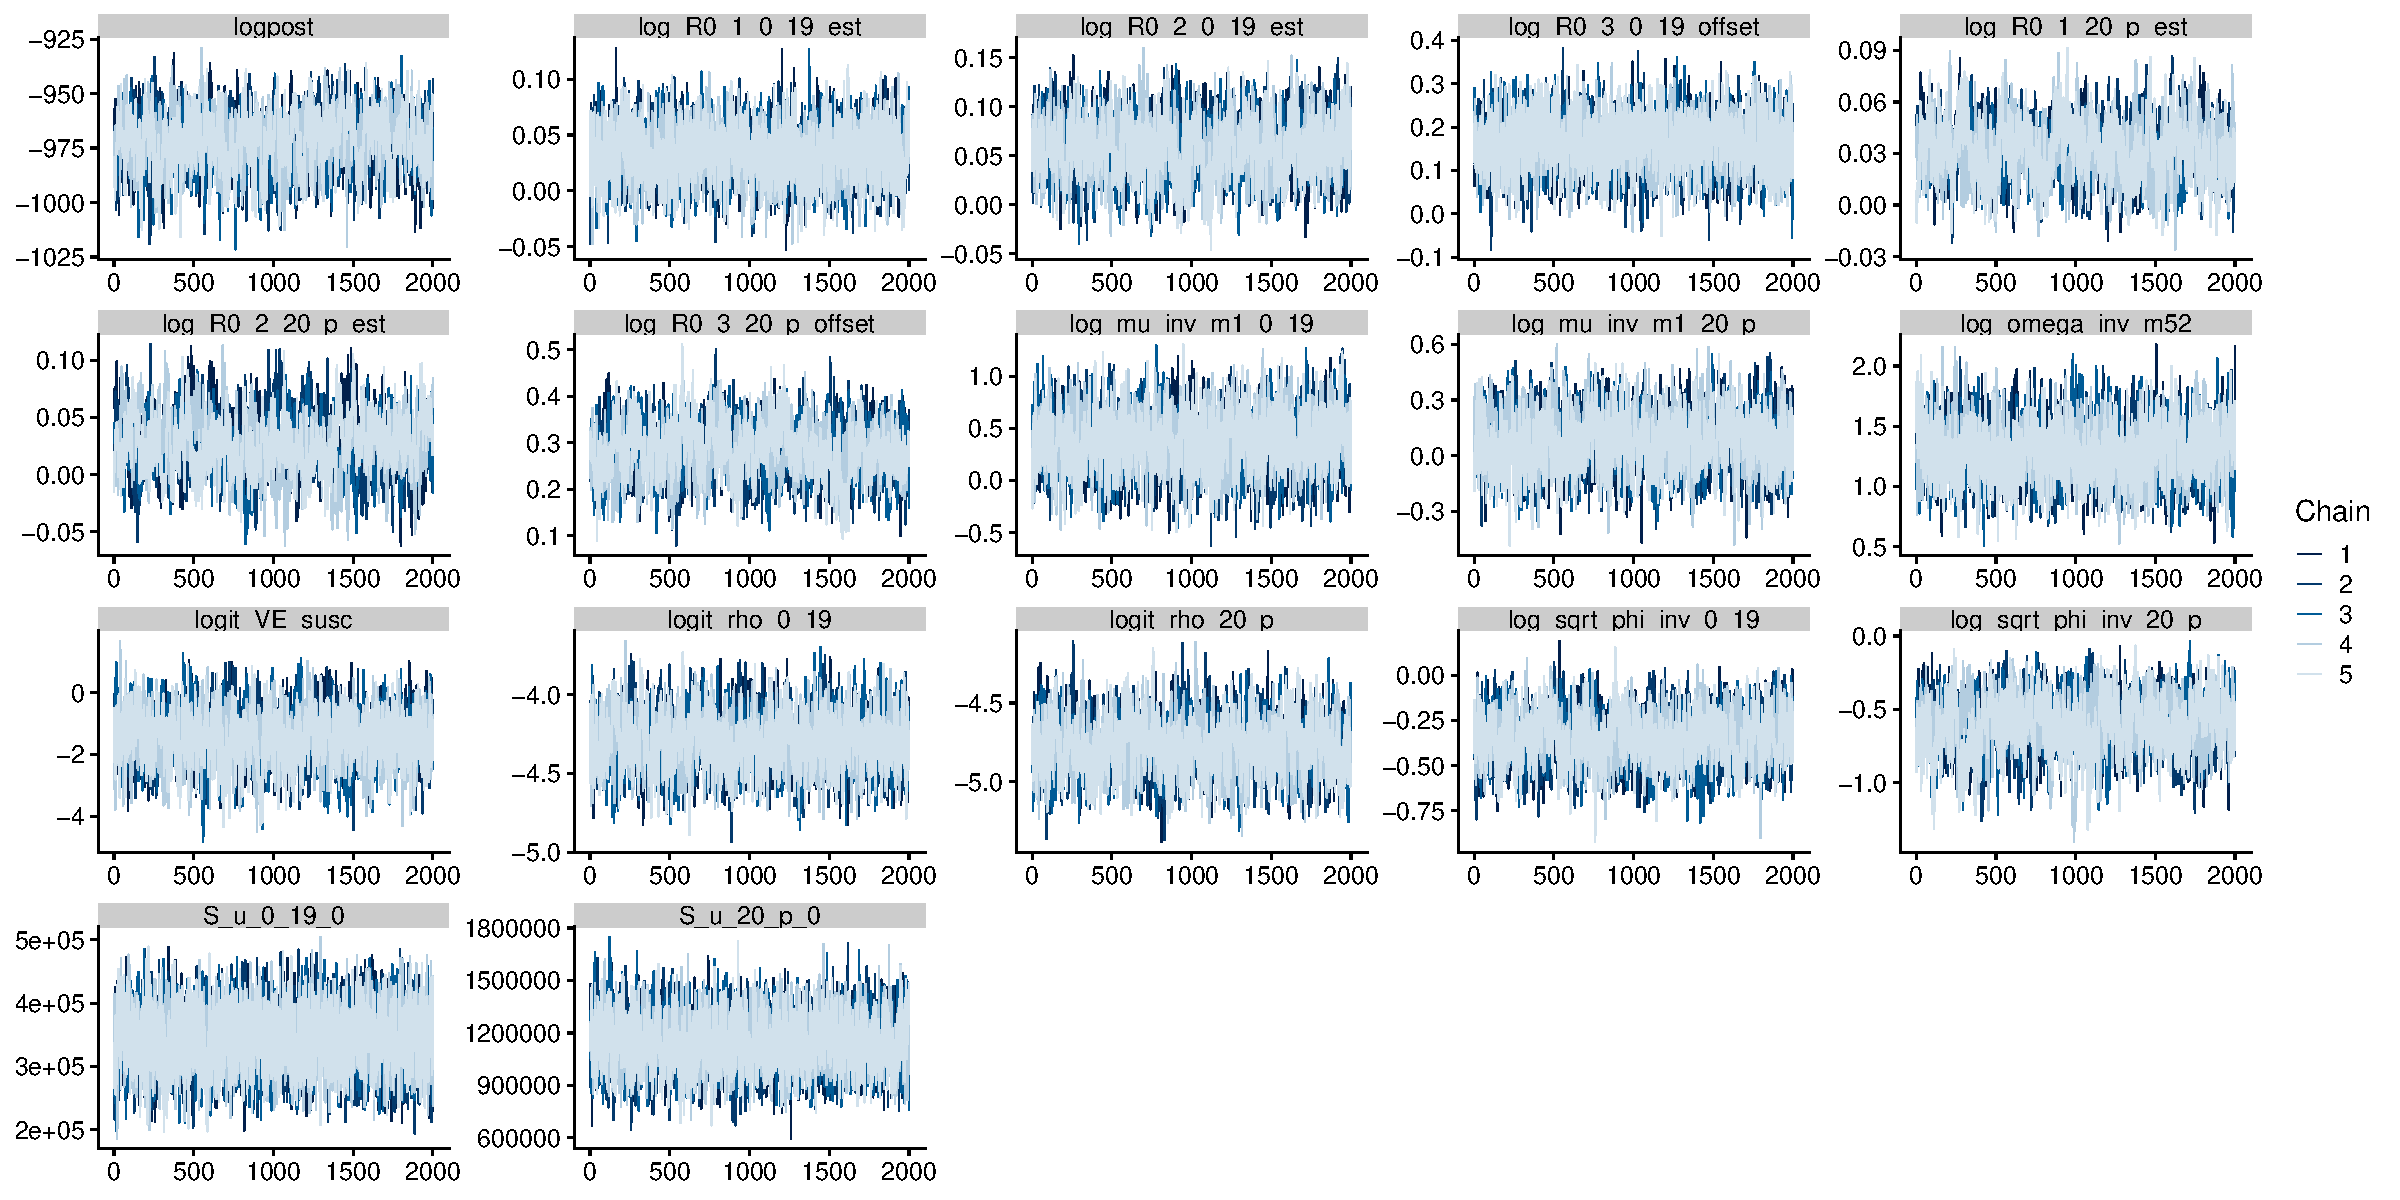
\includegraphics[width=\linewidth]{figures/flu_traces_const_ode}
	\caption{Posterior traceplots for a stratified SIRS ODE model with piecewise--homogeneous dynamics fit to data from the A(H1N1) influenza pandemic in Finland.}
	\label{fig:fluconstodetraces}
\end{sidewaysfigure}


\begin{sidewaysfigure}[htbp]
	\centering
	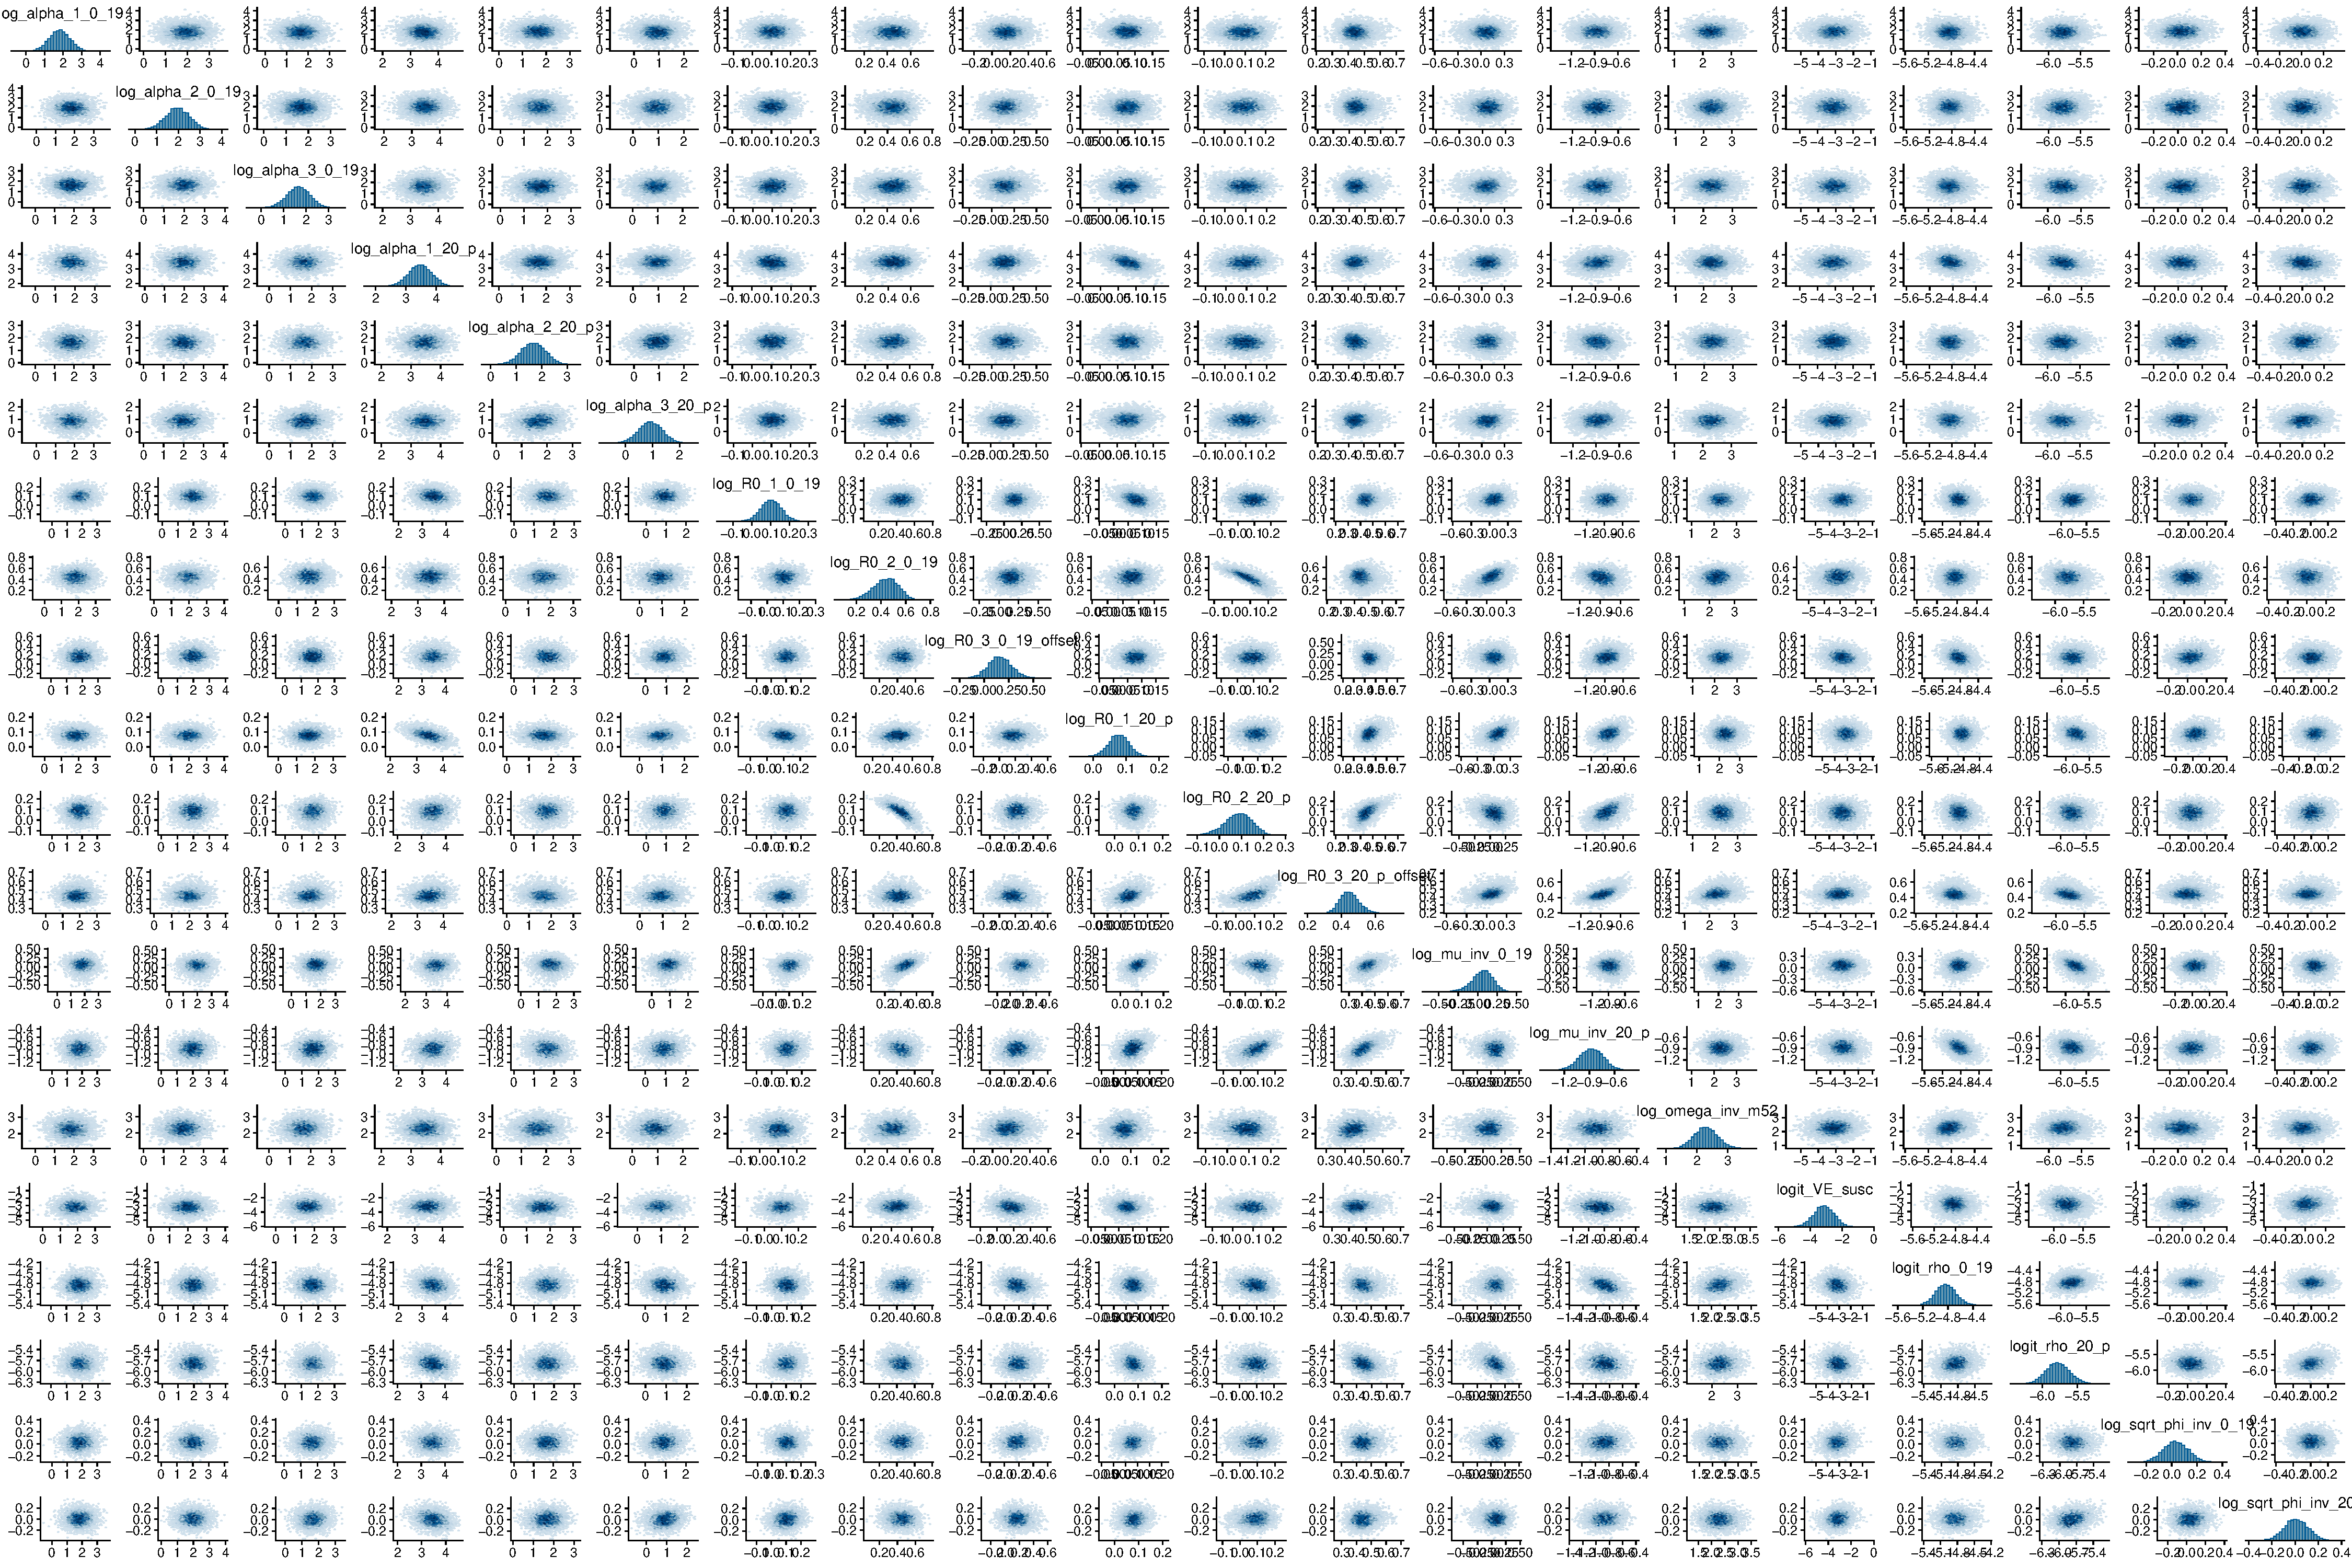
\includegraphics[width=\linewidth]{figures/flu_const_pairs}
	\caption{Histograms and pairwise scatterplots of posterior samples for the parameters of a stratified SIRS ODE model with piecewise homogeneous dynamics that were sampled via MVNSS. The model was fit to data from the A(H1N1) influenza pandemic in Finland.}
	\label{fig:fluconstpairs}
\end{sidewaysfigure}